\documentclass[a4paper]{article}
\usepackage{amsmath,amssymb,float,geometry,graphicx,minted,pgfplots,tikz,xcolor}
% \captionsetup[figure]{labelsep=period}
% \captionsetup[table]{labelsep=period}
\geometry{left=3.5cm,right=3.5cm,top=3.3cm,bottom=3.3cm}
\renewcommand\thesection{\arabic{section}}
\begin{document}
\begin{center}
\huge
\textbf{VE320\\Intro to Semiconductor Devices\\}
\Large
\vspace{30pt}
\uppercase{Homework 5 Attached Pages}\\
\vspace{5pt}\today\\
\vspace{5pt}
Yihua Liu 518021910998
\vspace{5pt}
\rule[-10pt]{.97\linewidth}{0.05em}
\end{center}
\begin{figure}[H]
    \centering
    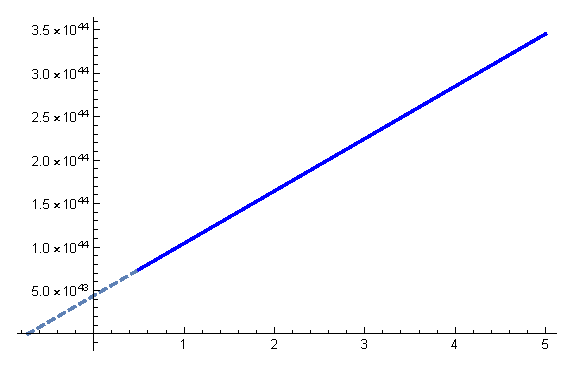
\includegraphics[width=1\textwidth]{1.eps}
    \caption{2(c).}
\end{figure}
\begin{figure}[H]
    \centering
    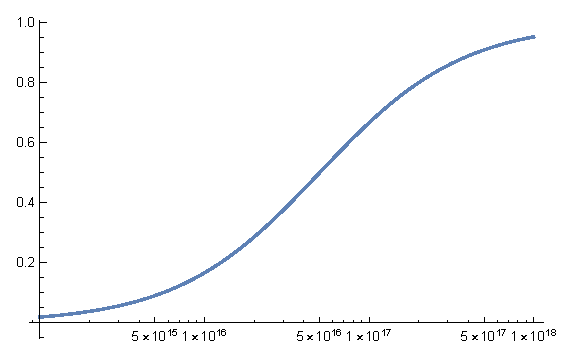
\includegraphics[width=1\textwidth]{2.eps}
    \caption{5}
\end{figure}
\begin{figure}[H]
    \centering
    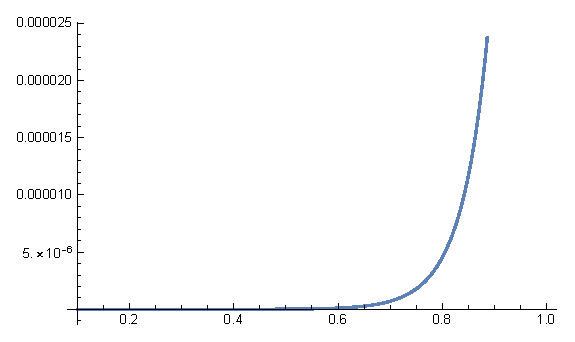
\includegraphics[width=1\textwidth]{3.eps}
    \caption{8 - the diode forward-bias current include including recombination current.}
\end{figure}
\begin{figure}[H]
    \centering
    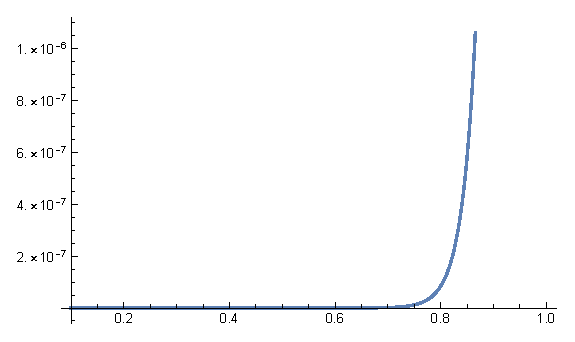
\includegraphics[width=1\textwidth]{4.eps}
    \caption{8 - an ideal diode.}
\end{figure}
\end{document}